\documentclass{article}



\usepackage{arxiv}

\usepackage[utf8]{inputenc} % allow utf-8 input
\usepackage[T1]{fontenc}    % use 8-bit T1 fonts
\usepackage{hyperref}       % hyperlinks
\usepackage{url}            % simple URL typesetting
\usepackage{booktabs}       % professional-quality tables
\usepackage{amsfonts}       % blackboard math symbols
\usepackage{nicefrac}       % compact symbols for 1/2, etc.
\usepackage{microtype}      % microtypography
\usepackage{lipsum}		% Can be removed after putting your text content
\usepackage{graphicx}
\usepackage{natbib}
\usepackage{array}
\usepackage{doi}
\usepackage{physics}
\setlength{\parindent}{0pt}


\title{Calculating Gradients In Quantum Neural Network}

\author{F08222011 Chen, Yi-An\\
	Department of Physics\\
	National Taiwan University\\
	\texttt{r08222011@gmail.com} \\
}

% Uncomment to remove the date
\date{}

% Uncomment to override  the `A preprint' in the header
\renewcommand{\headeright}{Quantum Computation and Quantum Information}
\renewcommand{\undertitle}{}
\renewcommand{\shorttitle}{}

%%% Add PDF metadata to help others organize their library
%%% Once the PDF is generated, you can check the metadata with
%%% $ pdfinfo template.pdf
\hypersetup{
pdftitle={Parmeter-Shift Rule},
pdfsubject={Quantum Machine Learning},
pdfauthor={F08222011 Chen, Yi-An},
pdfkeywords={Quantum Machine Learning, Variational Quantum Circuit, Gradient Descent},
}

\begin{document}
\maketitle

\begin{abstract}
    
    It is hard to calculate the gradient for Variational Quantum Circuit (VQC) with classical differentiation method. Especially in NISQ era, the noise of gates or measurements will cause a huge error on classical differentiation method. We use Parameter-Shift Rule (PSR) proposed by \citet{1905.13311} to calculate the gradient in a more quantum-efficient way. 
    
\end{abstract}


% keywords can be removed
\keywords{Quantum Machine Learning \and Variational Quantum Circuit \and Gradient Descent}


\section{Introduction}
Deep learning have been used in many fields, such as data classification, Natural Language Processing (NLP), regression, etc. Those different problems use different structures of deep neural network, but the basic ideas are the same: reducing the loss function by tuning parameters. There are several ways to reduce the loss, probably the most familiar one is to use Gradient Descent (GD) method. GD requires the gradient of the tunable parameters (training parameters), and it can be calculated easily with classical computers, e.g. finite difference method or back propagation.

In recent years, researchers have tried to use quantum computers to implement machine learning. The most intuitive way is to implement machine learning using quantum circuits, one of the example is to implement deep neural network with a quantum computer, which is the basic idea of "Variational Quantum Circuit" (VQC) by \citet{VQE}. However, if we want to implement "Gradient Descent Method" with a quantum computer, it's hard to calculate the gradients in NISQ era with classical differentiation method such as finite difference method. We now introduce a method called "Parameter-Shift Rule" (PSR) proposed by \citet{1905.13311}. Unlike most of the classical differentiation method, PSR gives an analytic solution based on the natural structure of Pauli rotation gates. In the following sections, we give a simple derivation of PSR.

\section{Problem and Methodology}
In this section, we first briefly review the basic ideas of classical neural network. Then we will see how we implement neural network on a quantum computer, e.g. VQC, using quantum circuits. Finally, we use PSR to calculate the gradients.

\subsection{Review of Classical Neural Network}
\begin{figure}
    \centering
    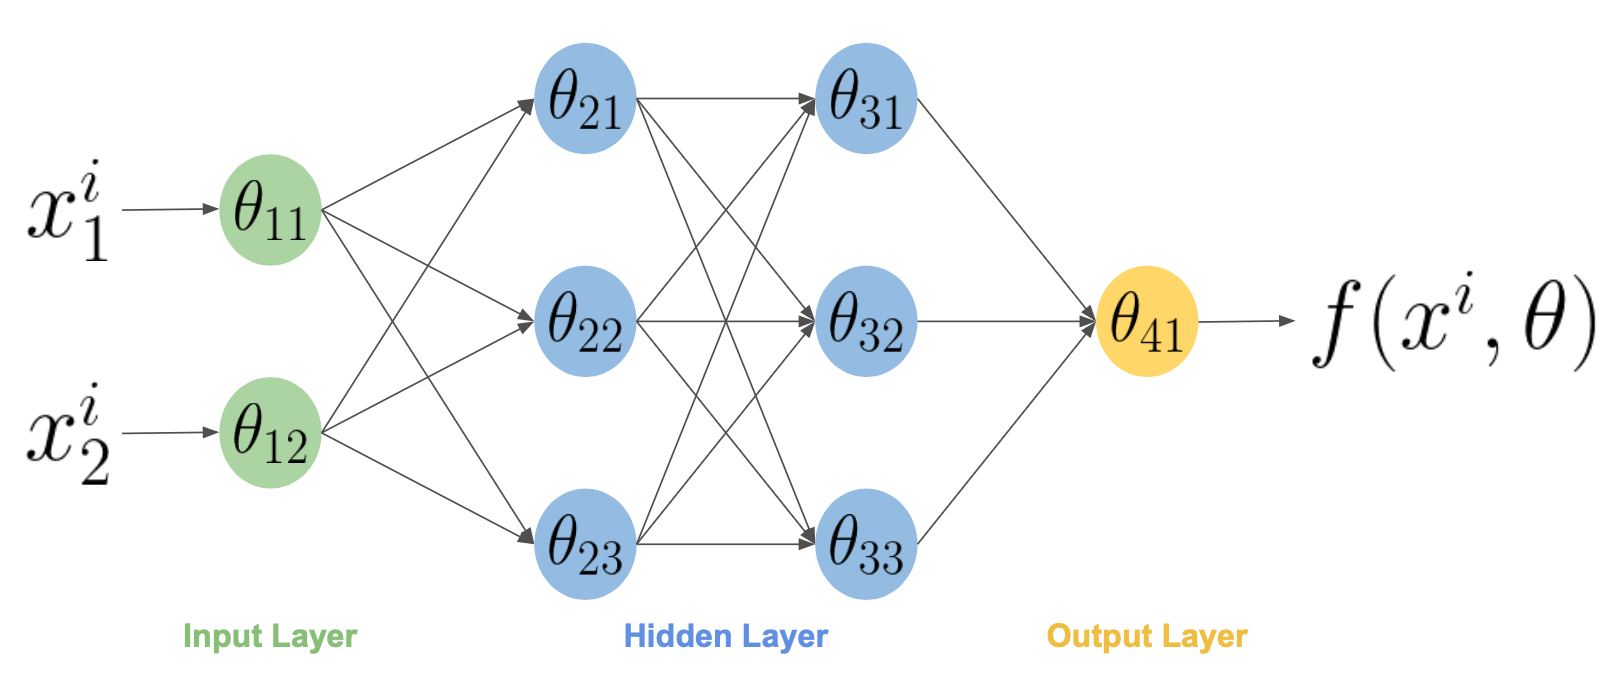
\includegraphics[scale=0.4]{dnn.png}
    \caption{Basic structure of a classical neural network. The circles are the neurons, each neuron will have one or more tunable (trainable) parameters. When feeding in a data $x^i$, it will output a value $f(x^i,\theta)$}
    \label{dnn}
\end{figure}
Neural network consists of neurons (circles on Fig.\ref{dnn}), briefly speaking, one can think of the number of neurons as the ability or complexity of the function we can learn. Each neuron consists of certain number of parameters $\theta$, we call them tunable parameters or trainable parameters, or simply parameters if there is no confusion in the context. The initial values of parameters is randomly chosen, e.g., can be generated from uniform distribution or Gaussian distribution.

In the following sections, we deal with classification problems. Suppose we have a dataset \{$(x^i,y^i)$\} for $i$ from $1$ to $N$, where $x^i$ is the feature vector of $i$-th data, $x^i$ can be multi-dimension (the features will be denoted as $x^i_1$, $x^i_2$, ...). The $y^i$ is usually called the true value or label of the $i$-th data. When we feed a data ($x^i$ in Fig.\ref{dnn}) into the neural network, it will feed forward the data and output a predicted value depends on the parameters $\theta$. One can define a loss function to quantify the error of the predicted values. For instance, we use the squared loss function defined as
\begin{equation}
    L(\theta)=\sum^{N}_{i=1}(f(x^i,\theta)-y^i)^2  .
\end{equation}
Intuitively, the smaller the loss, the more accurate the function $f$. In order to tune the parameters to reduce the loss, we use the famous "Gradient Descent" (GD) method. The basic idea is to update the parameters by
\begin{equation}
    \theta \rightarrow \theta - \lambda \nabla L(\theta)
\end{equation}
where $\lambda$ is a positive real number called the learning rate, it controls how fast we update our parameters. We can further expand the gradient as
\begin{equation} \label{gL}
    \nabla L(\theta)=\sum^{N}_{i=1}2(f(x^i,\theta)-u^i)\frac{\partial f}{\partial \theta}.
\end{equation}

\subsection{Introduction to Quantum Neural Network}
\begin{figure}
    \centering
    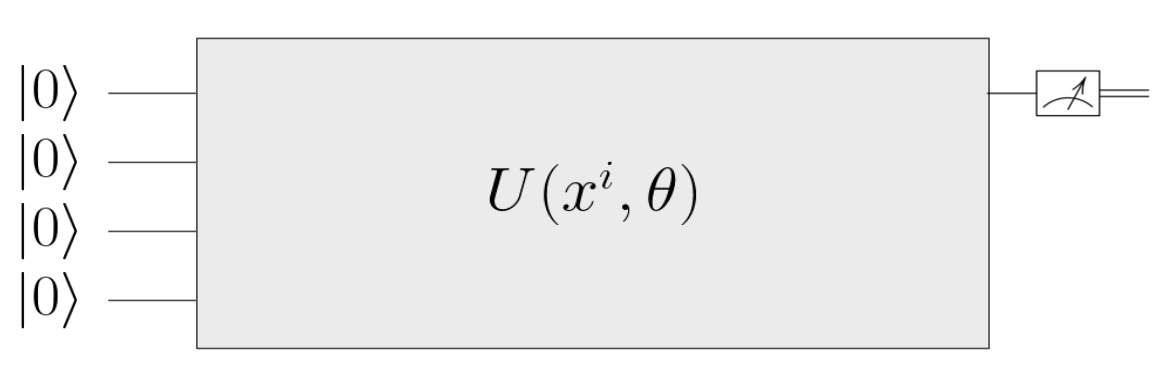
\includegraphics[scale=0.5]{vqc.png}
    \caption{The basic idea of VQC is to implement the quantum circuit with unitary gates that contain parameters. To analog the classical neural net work, we can take the measurement as the output value.}
    \label{vqc}
\end{figure}
One of the most famous example to apply the idea of neural network using quantum computers is "Variational Quantum Circuit" (VQC), proposed first in the work of \citet{VQE}. The basic idea of VQC is to use unitary gates with tunable parameters (see Fig.\ref{vqc}). Analogous to classical neural network, one can take the measurement as the output value (prediction). An example will be showed in our experiment.

However, if we want to optimize the parameters using GD method, we need to calculate the gradients. But since in the NISQ era, quantum computers may have noise, which cause a bad precision and a huge error on calculating gradients using classical differentiation method such as finite different method. To circumvent this problem, we certainly need a new way to calculate gradient on quantum computers. Fortunately, if our parameters are encoded with some special structures, e.g., Pauli rotation gates, then we can calculate the gradient with high precision. This method is called "Parameter-Shift Rule"(PSR) proposed by \citet{1905.13311}. Suppose we have a Pauli rotation gate $R(\theta)=e^{-i\frac{\theta}{2}\sigma}$ for some Pauli matrix $\sigma$ with a parameter $\theta$ in our circuit. Squeeze other gates into $A$ and $\ket{\psi}$, and
focus on this Pauli rotation gate, we can write our function as
\begin{equation} \label{vqc_f}
    f(x^i,\theta)=\bra{\psi}R^\dagger(\theta)AR(\theta)\ket{\psi},
\end{equation}
where $\ket{\psi}$ is the state operated by gates before $R(\theta)$, and $A$ is the gates and measurements after $R(\theta)$. Surprisingly, the gradient of $f$ can be calculated by
\begin{equation} \label{vqc_gf}
    \frac{\partial f}{\partial \theta}=\frac{1}{2}[f(x^i, \theta+\frac{\pi}{2})-f(x^i, \theta-\frac{\pi}{2})].
\end{equation}
The important thing is that this is an exact value, not an approximation! What's more? We plus and minus the parameter with $\pi/2$, this is a huge difference with finite difference method, and can be used in the NISQ era. Finally, we plug Eq.\ref{vqc_gf} into Eq.\ref{gL} in order to update the parameters using GD method.

\section{Result and Analysis}
\subsection{Experiment Setup}
We demonstrate the power of PSR by training a small model. We use the traditional dataset known as Iris Data, provided by \cite{iris}. There are 3 different classes in Iris dataset, each with 50 data. Each data has 4 features, we use Principal Component Analysis (PCA) to reduce the dimension of features from 4 to 2. We then choose 2 of the classes to setup a classification problem. The dataset will be split into 90 training data and 10 testing data (each class will has 45 training data and 5 testing data).
\begin{figure}
    \centering
    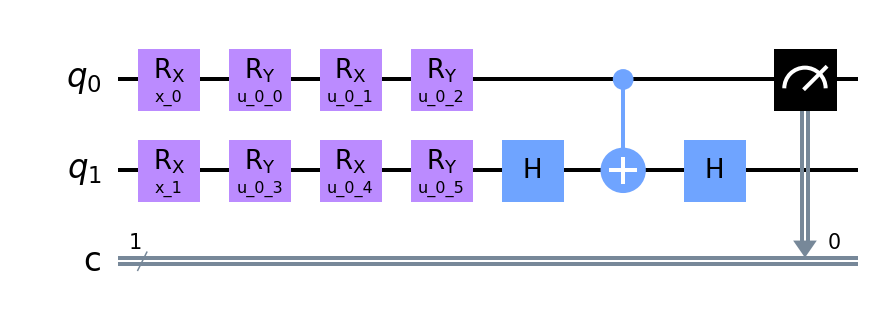
\includegraphics[scale=0.5]{vqc_2.png}
    \caption{Structure of VQC. The data ($x^i_1$ and $x^i_2$ are the two PCA features of each data) is encoded in the angle of rotation gates. Then the circuit will be followed by some parametrized gates (with tunable parameters $\theta$) and entangling gates. Finally, we only measure the first qubit in the Z-basis as the output value.}
    \label{vqc_2}
\end{figure}
The structure of our VQC is provided in Fig.\ref{vqc_2}. We use rotation angle to encode our data. Since the argument for rotation gates has a period in $[0,2\pi]$, we shift and scale the Iris data into $[0,\pi]$, so the state will be prepared between $\ket{0}$ and $\ket{1}$. After encoding gates, we operate a series of Pauli rotation gates with tunable parameters, then we also apply Hadamard gates with CNOT gate to get a controlled-Z gate. Finally, the first qubit will be measured in the Z-basis. We set the output value to be the expectation value of number of measurements in $\ket{1}$, so the output value will be restricted between $[0,1]$.

\begin{table}
    \begin{center}
    \caption{Hyper-parameters we use in our experiment.}
    \label{hyperpara}
    \begin{tabular}{ | c | c | }
        \hline
        measurement shots & 128 and 1024 \\
        \hline
        number of qubits & 2 \\ 
        \hline
        training epochs & 10 \\
        \hline
        learning rate $\lambda$ & 1 \\
        \hline
        noise rate & 0.1 \\
        \hline
    \end{tabular}
    \end{center}
\end{table}

The VQC will be trained with total 10 epochs. For optimization, we use "Stochastic Gradient Descent" (SGD) method, simply a simplified version of GD method. In SGD, we randomly choose 5 data out of training data and calculate the mean loss gradient to optimize the parameters $\theta$. Other hyper-parameters will be listed in Table \ref{hyperpara}.

\subsection{Experiment Result}

\begin{figure}
    \centering
    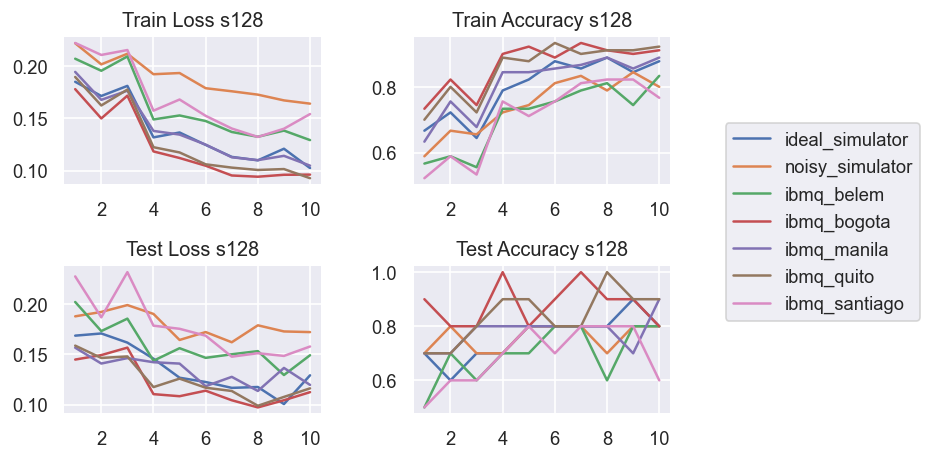
\includegraphics[scale=0.8]{s128.png}
    \caption{Results of training with shots=128}
    \label{s128}
\end{figure}
\begin{figure}
    \centering
    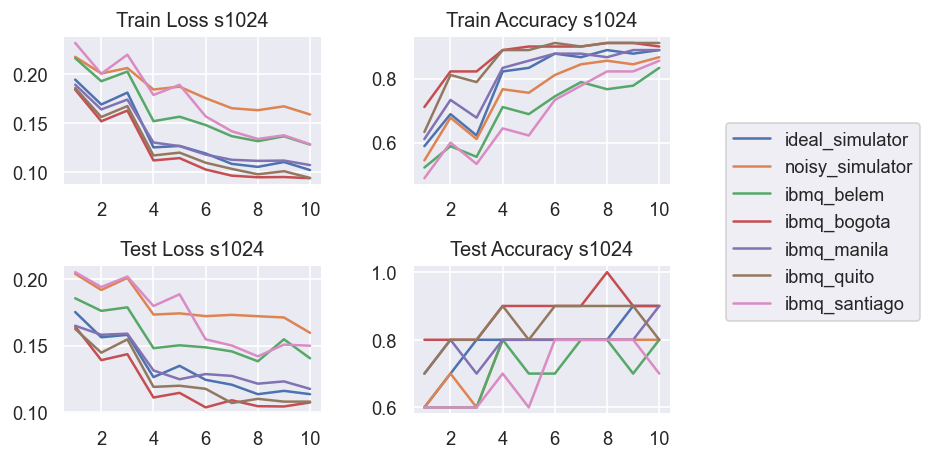
\includegraphics[scale=0.8]{s1024.png}
    \caption{Results of training with shots=1024}
    \label{s1024}
\end{figure}
We use Qiskit "qasm\_simulator" for our simulation, including ideal simulator (noise-free) and noisy simulator (for detail, see github \url{https://github.com/r08222011/Qiskit\_Parameter\_Shift}). For real quantum computers, we choose 5-qubit quantum computers. We have successfully test on "ibmq\_belem", "ibmq\_bogota", "ibmq\_manila", "ibmq\_santiago" and "ibmq\_quito". The only one "ibmq\_lima" has too many queues to be wait, so we skip these two quantum computers.

Training results for shots 128 and shots 1024 can be found in Fig.\ref{s128} and Fig.\ref{s1024} respectively. We see that PSR works well both in simulator and real quantum computers, since they can both be trained successfully (meaning that the loss is reduced and the accuracy is increased). One interesting thing to be noticed is that "ibmq\_bogota" and "ibmq\_quito" perform even better than "ideal\_simulator", we think that it was just a coincidence.

\section{Discussion and Conclusion}

PSR is certainly a candidate for training a VQC, however, the (time and space) complexity should be discussed. Unlike the classical method such as back propagation, we can only calculate the gradient for a parameter at a time, which means the training time complexity is polynomial in the number of parameters. Also, to use PSR technique, one should obey the special structure of gates we use, such as Pauli rotation gates. The greatest advantage of PSR is that we calculate the gradient by shifting the parameters by $\pi/2$, unlike finite difference method, this is exact a value!

There are other techniques for training VQC such as data re-upload proposed by \citet{reupload}, we also implement this technique in our code. However, due to the restriction of the usage of IBM quantum computers, we didn't use this technique in our experiment.

\bibliographystyle{unsrtnat}
\bibliography{references}  %%% Uncomment this line and comment out the ``thebibliography'' section below to use the external .bib file (using bibtex) .


%%% Uncomment this section and comment out the \bibliography{references} line above to use inline references.
% \begin{thebibliography}{1}

% 	\bibitem{kour2014real}
% 	George Kour and Raid Saabne.
% 	\newblock Real-time segmentation of on-line handwritten arabic script.
% 	\newblock In {\em Frontiers in Handwriting Recognition (ICFHR), 2014 14th
% 			International Conference on}, pages 417--422. IEEE, 2014.

% 	\bibitem{kour2014fast}
% 	George Kour and Raid Saabne.
% 	\newblock Fast classification of handwritten on-line arabic characters.
% 	\newblock In {\em Soft Computing and Pattern Recognition (SoCPaR), 2014 6th
% 			International Conference of}, pages 312--318. IEEE, 2014.

% 	\bibitem{hadash2018estimate}
% 	Guy Hadash, Einat Kermany, Boaz Carmeli, Ofer Lavi, George Kour, and Alon
% 	Jacovi.
% 	\newblock Estimate and replace: A novel approach to integrating deep neural
% 	networks with existing applications.
% 	\newblock {\em arXiv preprint arXiv:1804.09028}, 2018.

% \end{thebibliography}



\end{document}